
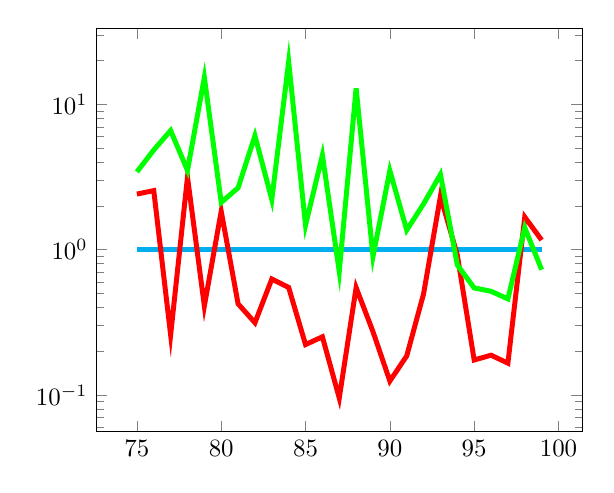
\begin{tikzpicture}[scale=0.9]
\begin{semilogyaxis}
\addplot[color=cyan,line width=2pt] coordinates {(75,1.0)(76,1.0)(77,1.0)(78,1.0)(79,1.0)(80,1.0)(81,1.0)(82,1.0)(83,1.0)(84,1.0)(85,1.0)(86,1.0)(87,1.0)(88,1.0)(89,1.0)(90,1.0)(91,1.0)(92,1.0)(93,1.0)(94,1.0)(95,1.0)(96,1.0)(97,1.0)(98,1.0)(99,1.0)};
\addplot[color=red,line width=2pt] coordinates {(75,2.410847881807989)(76,2.5457749770250757)(77,0.25875291639056497)(78,3.1538255653371072)(79,0.40914831348020925)(80,1.8348344752326904)(81,0.4236440408897098)(82,0.3139592144919407)(83,0.6275941412047091)(84,0.5489502985409658)(85,0.22198087341701245)(86,0.2511714249874563)(87,0.0951755293775357)(88,0.5475864419434875)(89,0.2722565358450827)(90,0.12459399664664772)(91,0.18545741218612302)(92,0.496251982354764)(93,2.326901930674097)(94,0.9179972423914265)(95,0.17390779168522613)(96,0.1876664503441743)(97,0.16540456617039065)(98,1.6742764189227437)(99,1.163206030464955)};
\addplot[color=green,line width=2pt] coordinates {(75,3.424003824367273)(76,4.8461987659183405)(77,6.598777645024372)(78,3.5065852313296593)(79,15.316887681805934)(80,2.112189377757193)(81,2.661242708097212)(82,6.076720010134581)(83,2.2113319543182635)(84,19.60873616147567)(85,1.471593651652065)(86,4.463473809235008)(87,0.7068995160954853)(88,12.888760246393383)(89,0.8974645552537704)(90,3.496656702251482)(91,1.3619659242883513)(92,2.064012855684573)(93,3.2936446527999026)(94,0.7836925325616764)(95,0.5447968562437377)(96,0.5165729620074676)(97,0.4580289311077836)(98,1.4150928885902936)(99,0.7277670053001903)};

\end{semilogyaxis}
\end{tikzpicture}
